\section{Двухвыборочная задача}

Чтобы понять обозначения (8.2), рассмотрим данные о мышах в таблице 2.1. Вероятностную модель $P$ можно представить как пару распределений вероятностей $F$ и $G$, первое для экспериментальной группы и второе для контрольной группы
\begin{equation}
	P = (F, G).
\end{equation}

Пусть $\textbf{z} = (z_1, z_2, \ldots, z_m)$ обозначает экспериментальные наблюдения, а $\textbf{y} = (y_1, y_2, \ldots, y_n)$ обозначает контрольные наблюдения с $n = 7$ и $m = 9$. Тогда наблюдаемые данные включают $\textbf{z}$ и $\textbf{y}$
\begin{equation}
	\textbf{x} = (\textbf{z}, \textbf{y}).
\end{equation}
Можем представить себе $\textbf{x}$ как $16$-мерный вектор, если мы помним, что семь элементов из $F$, девять --- из $G$. Отображение $P \to \bf{x}$ описывается следующим образом:
\begin{equation}
	F \to \textbf{z} \text{ независимо от } G \to \textbf{y}.
\end{equation}
Другими словами, $\textbf{z}$ --- это случайная выборка размера $7$ из $F$, $\textbf{y}$ --- случайная выборка размера $9$ из $G$, причем $\textbf{z}$ и $\textbf{y}$ взаимно независимы друг от друга. Такая постановка называется \textit{двухвыборочной задачей}. 

В этом случае легко оценить вероятностный механизм $P$. Пусть $\hat{F}$ и $\hat{G}$~--- эмпирические распределения, основанные на $\textbf{z}$ и $\textbf{y}$ соответственно. Тогда естественная оценка $P = (F, G)$ такова:
\begin{equation}
	\hat{P} = (\hat{F}, \hat{G}).
\end{equation}

После получения $\hat{P}$ определение бутстреп выборки $\textbf{x}^*$ очевидно, стрелка в выражении
\begin{equation}
	\hat{P} \to \textbf{x}^*
\end{equation}
должна означать то же самое, что и стрелка в $P \to \textbf{x}$, (8.2). В двухвыборочной задаче (8.5) мы имеем $\textbf{x}^* = (\textbf{z}^*, \textbf{y}^*)$, где
\begin{equation}
	\hat{F} \to \textbf{z}^* \text{ независимо от } \hat{G} \to \textbf{y}^*.
\end{equation}
Размеры выборки для $\textbf{z}^*$ и $\textbf{y}^*$ такие же, как для $\textbf{z}$ и $\textbf{y}$ соответственно.

На рисунке 8.2 показана гистограмма $B = 1400$ бутстреп репликаций статистики $\hat \theta$
 \begin{align}
 	\hat{\theta} & = \hat{\mu}_z - \hat{\mu}_y = \bar{z} - \bar{y} = \notag \\
 	& = 86.86 - 56.22 = 30.63,
 \end{align}
где $\hat \theta$ --- разность в средних значениях экспериментальной и контрольной групп в данных о мышах. Эта статистика оценивает параметр
\begin{equation}
	\theta = \mu_z - \mu_y = \text{E}_f(z) - \text{E}_G(y).
\end{equation}
Если $\theta$ действительно намного больше $0$, как, по-видимому, указывает (8.9), то экспериментальная группа показывает гораздо лучший результат по сравнению с контрольной группой. Однако бутстреп оценка стандартной ошибки для $\hat{\theta} = 30.63$ это
\begin{equation}
	\widehat{\text{se}}_{1400} = \left\{ \sum_{b=1}^{1400} [ \hat{\theta}^*(b) - \hat{\theta}^*(\cdot) ]^2 / 1399 \right\}^{1/2} = 26.85,
\end{equation}
поэтому $\hat{\theta}$ всего лишь на $1.14$ стандартной ошибки больше нуля, $1.14 = 30.63 / 26.85$. Обычно такой результат не считается убедительным доказательством того, что истинное значение $\theta$ больше $0$.

Бутстреп репликации $\hat{\theta}^*$ были получены при помощи генератора случайных чисел для соблюдения независимости (8.8). Каждая бутстреп выборка $\textbf{x}^*$ вычислена следующим образом
\begin{equation}
	\textbf{x}^* = (\textbf{z}^*, \textbf{y}^*) = (z_{i_1}, z_{i_2}, \ldots, z_{i_7}, y_{j_1}, y_{j_2}, \ldots, y_{j_9}),
\end{equation}

\noindent где $(i_1, i_2, \ldots, i_7)$ есть случайная выборка размера $7$ из целых чисел $1,2,\ldots,7$, а $(j_1, j_2, \ldots, j_g)$ есть независимо выбранная случайная выборка размера $9$ из целых чисел $1, 2, \ldots, 9$. Например, первая бутстреп выборка $(i_1, i_2, \ldots, i_7) = (7,3,1,2,7,6,3)$ и $(j_1, j_2, \ldots, j_9) = (7,8,2,9,6,7,8,4,2)$.

Стандартная ошибка $\theta$ может быть записана как $\text{se}_P(\hat{\theta})$, чтобы подчеркнуть тот факт, что она зависит от неизвестного вероятностного механизма $P = (F, G)$. Бутстреп оценка $\text{se}_P(\hat{\theta})$ --- это оценка методом подстановки
\begin{equation}
	\text{se}_{\hat{P}}(\hat{\theta}^*) = \{ \text{var}_{\hat{P}}(\bar{z}^* - \bar{y}^*) \}^{1/2}.
\end{equation}
Как и в главе 6, мы аппроксимируем идеальную бутстреп оценку $\text{se}_{\hat{P}}(\hat{\theta}^*)$ при помощи $\widehat{\text{se}}_B$ из уравнения (6.6), в данном случае при $B = 1400$. Тот факт, что $\hat{\theta}^*$ вычисляется из двух выборок, $\textbf{z}^*$ и $\textbf{y}^*$ не влияет на определение (6.6), а именно $\widehat{\text{se}}_B = \left\{ \sum_{b=1}^{B} [\hat{\theta}^*(b) - \hat{\theta}^*(\cdot)]^2/(B-1) \right\}^{1/2}$.

\noindent
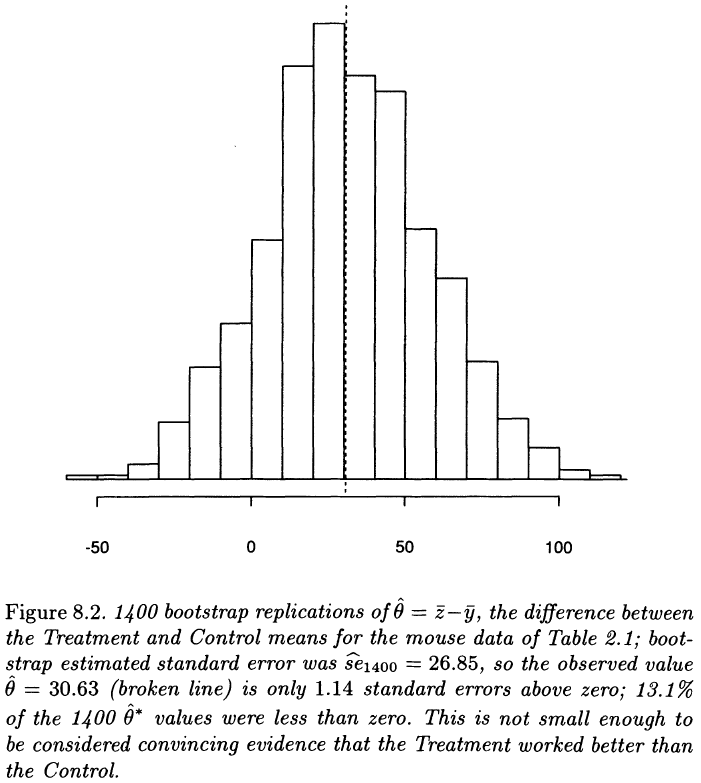
\includegraphics[width=\linewidth]{8/f82}
\newline